	
\subsubsection{20.10.14}

\begin{enumerate}
	\item Время начала и окончания собрания:
	20:30 - 21:30
	\item Цели собрания:
	\begin{enumerate}
	  \item Устранить баг сервопривода.
	  
	  \item Закрепить ребра жесткости на подъемнике.
	  
    \end{enumerate}
    
	\item Проделанная работа:
	\begin{enumerate}
	  \item Для устранения бага с сервоприводом мы попробовали сделать так, чтобы перед остановкой он немного прокручивался назад.Однако это ни к чему не привело.
      
      \item Приобретенный Г-образный профиль распилен на уголки нужной длины.
      
      \item Ребра жесткости для подъемника изготовлены. Одно из них установлено на работа.
      
      \begin{figure}[H]
      	\begin{minipage}[h]{0.47\linewidth}
        	\center{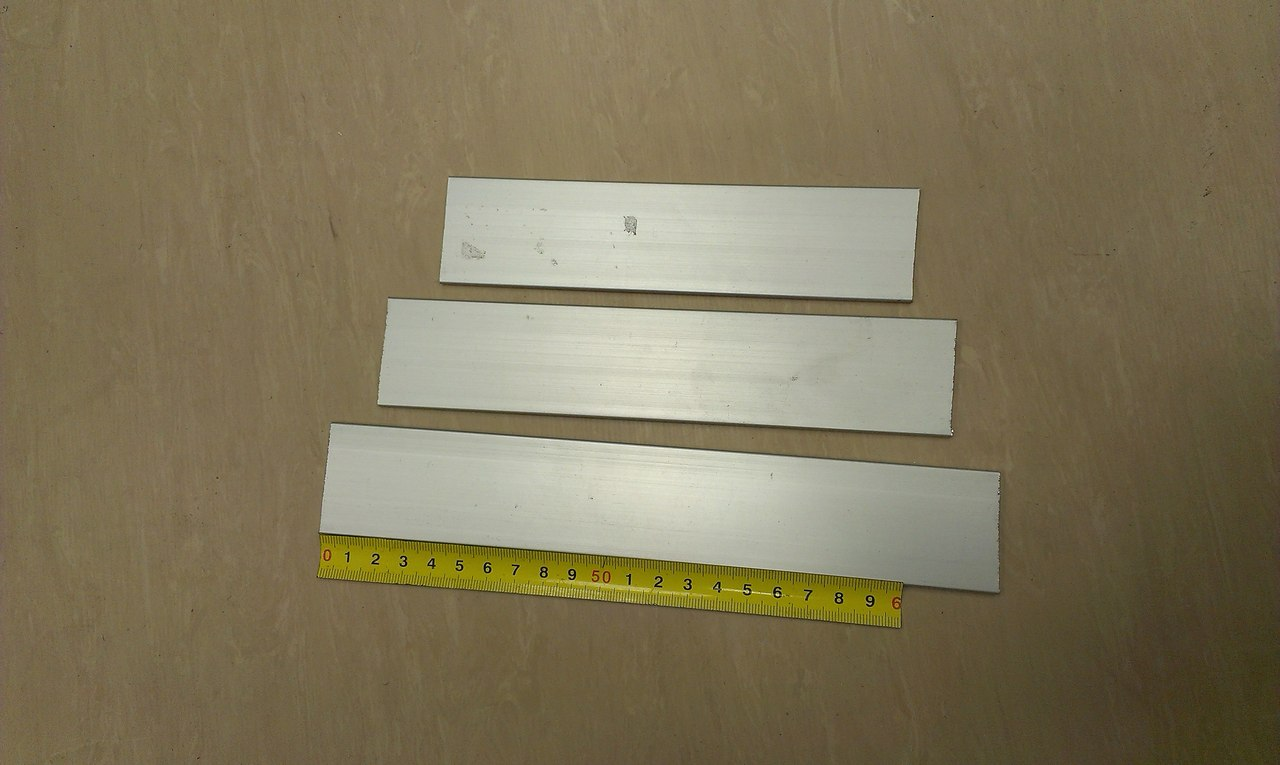
\includegraphics[scale=0.3]{days/images/0NsjR-ipcbw}}
      		\caption{Ребра жесткости}  
      	\end{minipage}
      	\hfill
      	\begin{minipage}[h]{0.47\linewidth}
      		\center{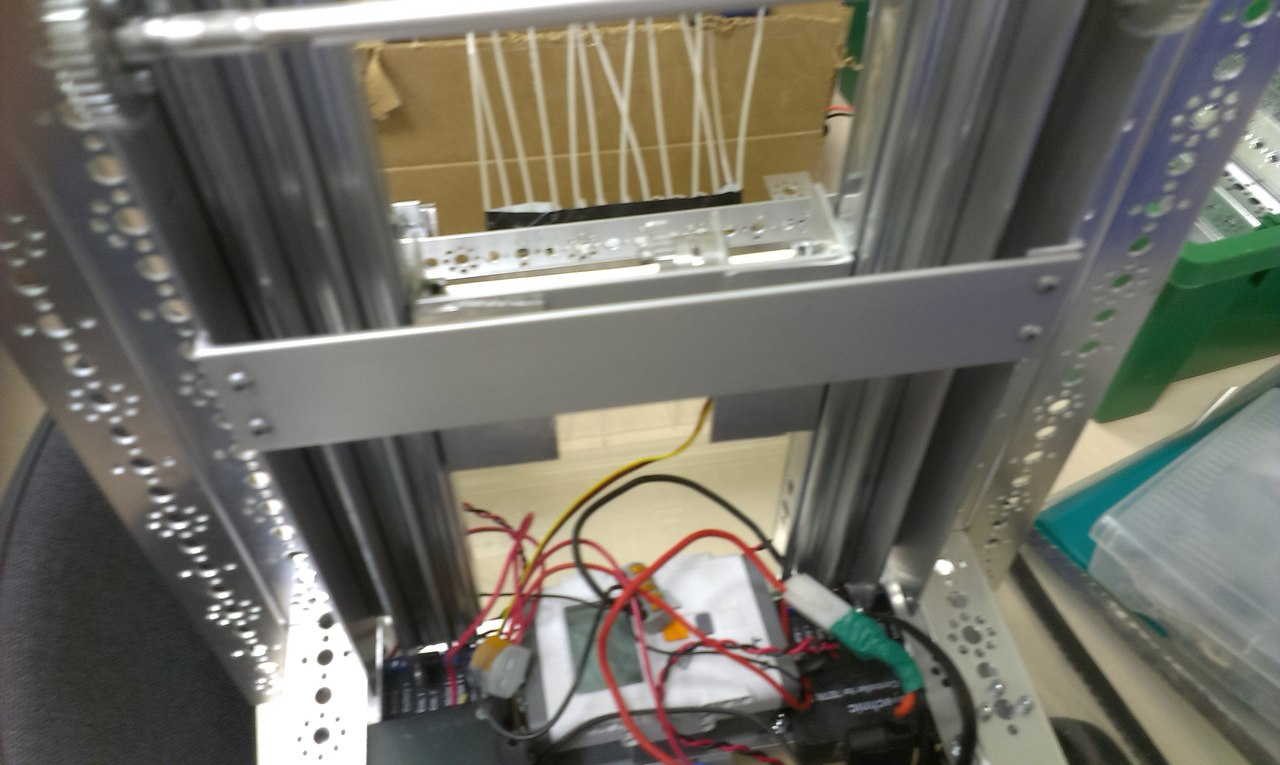
\includegraphics[scale=0.2]{days/images/XBmSlbH4MSc}}
      		\caption{Ребро жесткости, установленное на робота}
      	\end{minipage}
      \end{figure}
      
      \item Сегодня до нас дошли сведения, что 21 – 23 ноября будут проводиться соревнования FTC в Сочи. На обще-командном собрании было решено, что мы будем принимать в них участие. До среды каждый участник команды должен будет дать ответ, сможет ли он поехать в Сочи.
      
    \end{enumerate}
    
	\item Итоги собрания: 
	\begin{enumerate}
	  \item Ошибка сервопривода не устранена.
	  
      \item Все готово для закрепления ребер жесткости на направляющие подъемника.
      
      \item Одно ребро жесткости установлено.
      
    \end{enumerate}
    
	\item Задачи для последующих собраний:
	\begin{enumerate}
	  \item Закончить закрепление ребер жесткости на подъемник.
	  
	  \item Устранить ошибку сервопривода.
	  
	  \item	Решить до среды, каким составом наша команда поедет в Сочи.
	  
    \end{enumerate}     
\end{enumerate}

\fillpage
